%% Creator: Inkscape inkscape 0.92.2, www.inkscape.org
%% PDF/EPS/PS + LaTeX output extension by Johan Engelen, 2010
%% Accompanies image file 'exp2.eps' (pdf, eps, ps)
%%
%% To include the image in your LaTeX document, write
%%   \input{<filename>.pdf_tex}
%%  instead of
%%   \includegraphics{<filename>.pdf}
%% To scale the image, write
%%   \def\svgwidth{<desired width>}
%%   \input{<filename>.pdf_tex}
%%  instead of
%%   \includegraphics[width=<desired width>]{<filename>.pdf}
%%
%% Images with a different path to the parent latex file can
%% be accessed with the `import' package (which may need to be
%% installed) using
%%   \usepackage{import}
%% in the preamble, and then including the image with
%%   \import{<path to file>}{<filename>.pdf_tex}
%% Alternatively, one can specify
%%   \graphicspath{{<path to file>/}}
%% 
%% For more information, please see info/svg-inkscape on CTAN:
%%   http://tug.ctan.org/tex-archive/info/svg-inkscape
%%
\begingroup%
  \makeatletter%
  \providecommand\color[2][]{%
    \errmessage{(Inkscape) Color is used for the text in Inkscape, but the package 'color.sty' is not loaded}%
    \renewcommand\color[2][]{}%
  }%
  \providecommand\transparent[1]{%
    \errmessage{(Inkscape) Transparency is used (non-zero) for the text in Inkscape, but the package 'transparent.sty' is not loaded}%
    \renewcommand\transparent[1]{}%
  }%
  \providecommand\rotatebox[2]{#2}%
  \ifx\svgwidth\undefined%
    \setlength{\unitlength}{735.9999816bp}%
    \ifx\svgscale\undefined%
      \relax%
    \else%
      \setlength{\unitlength}{\unitlength * \real{\svgscale}}%
    \fi%
  \else%
    \setlength{\unitlength}{\svgwidth}%
  \fi%
  \global\let\svgwidth\undefined%
  \global\let\svgscale\undefined%
  \makeatother%
  \begin{picture}(1,0.89972826)%
    \put(0,0){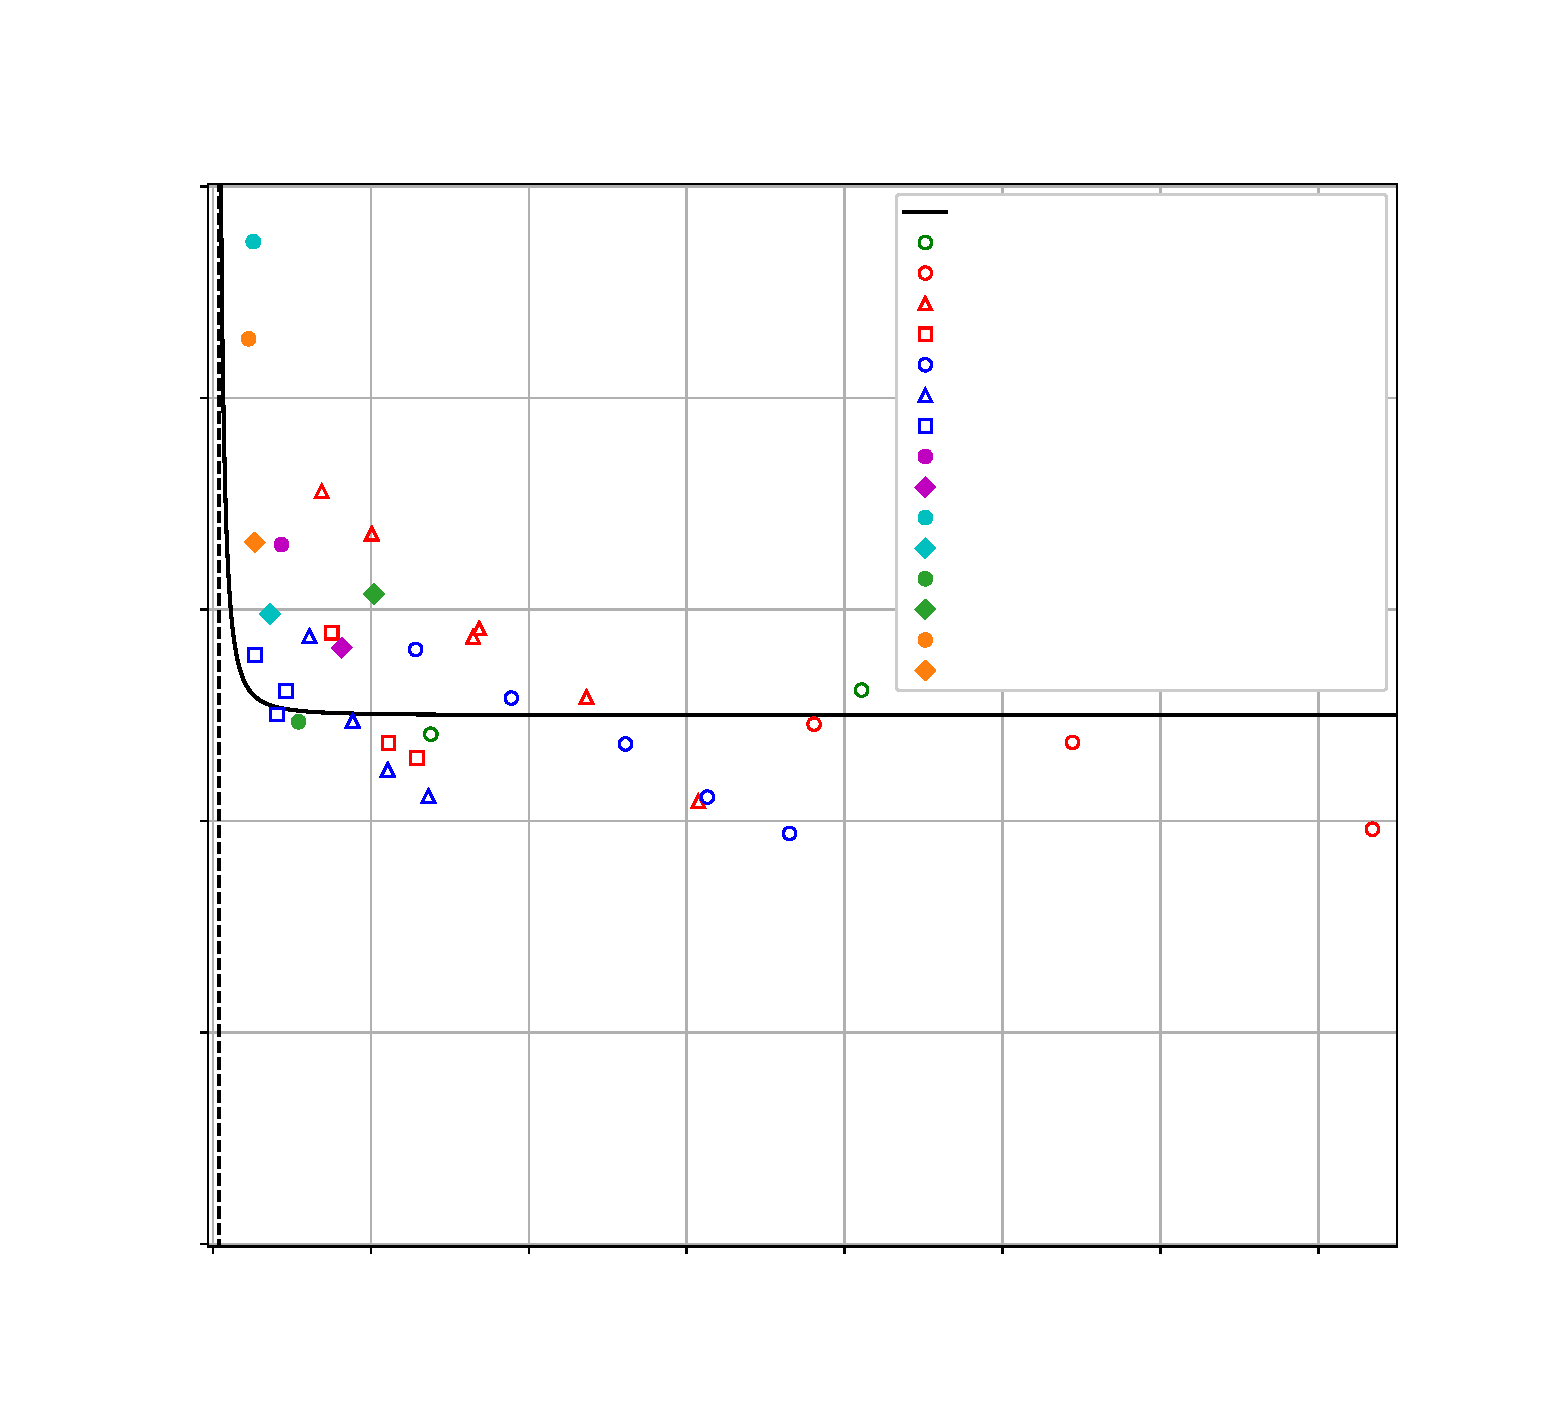
\includegraphics[width=\unitlength]{images_2ddl/exp2.eps}}%
    \put(0.12,0.065){\color[rgb]{0,0,0}\makebox(0,0)[lb]{\smash{0}}}%
    \put(0.21,0.065){\color[rgb]{0,0,0}\makebox(0,0)[lb]{\smash{20}}}%
    \put(0.31,0.065){\color[rgb]{0,0,0}\makebox(0,0)[lb]{\smash{40}}}%
    \put(0.41,0.065){\color[rgb]{0,0,0}\makebox(0,0)[lb]{\smash{60}}}%
    \put(0.52,0.065){\color[rgb]{0,0,0}\makebox(0,0)[lb]{\smash{80}}}%
    \put(0.61,0.065){\color[rgb]{0,0,0}\makebox(0,0)[lb]{\smash{100}}}%
    \put(0.72,0.065){\color[rgb]{0,0,0}\makebox(0,0)[lb]{\smash{120}}}%
    \put(0.82,0.065){\color[rgb]{0,0,0}\makebox(0,0)[lb]{\smash{140}}}%
    \put(0.067,0.0955428){\color[rgb]{0,0,0}\makebox(0,0)[lb]{\smash{0.0}}}%
    \put(0.067,0.23343071){\color[rgb]{0,0,0}\makebox(0,0)[lb]{\smash{0.2}}}%
    \put(0.067,0.37131929){\color[rgb]{0,0,0}\makebox(0,0)[lb]{\smash{0.4}}}%
    \put(0.067,0.50920788){\color[rgb]{0,0,0}\makebox(0,0)[lb]{\smash{0.6}}}%
    \put(0.067,0.64709511){\color[rgb]{0,0,0}\makebox(0,0)[lb]{\smash{0.8}}}%
    \put(0.067,0.7849837){\color[rgb]{0,0,0}\makebox(0,0)[lb]{\smash{1.0}}}%
    \put(0.045,0.38){\color[rgb]{0,0,0}\rotatebox{90}{\makebox(0,0)[lb]{\smash{$E_{p,g}/E_{tot}$}}}}%
    \put(0.45,0.02){\color[rgb]{0,0,0}\makebox(0,0)[lb]{\smash{$F/(m_r g)$}}}%
    \put(0.61703804,0.76890217){\color[rgb]{0,0,0}\makebox(0,0)[lb]{\smash{\tiny modèle théorique 2DDL}}}%
    \put(0.61703804,0.74896739){\color[rgb]{0,0,0}\makebox(0,0)[lb]{\smash{\tiny Y&K acier (120,30)}}}%
    \put(0.61703804,0.72903261){\color[rgb]{0,0,0}\makebox(0,0)[lb]{\smash{\tiny Y&K polyimide (125,10)}}}%
    \put(0.61703804,0.70909783){\color[rgb]{0,0,0}\makebox(0,0)[lb]{\smash{\tiny Y&K polyimide (125,15)}}}%
    \put(0.61703804,0.6891644){\color[rgb]{0,0,0}\makebox(0,0)[lb]{\smash{\tiny Y&K polyimide (125,20)}}}%
    \put(0.61703804,0.66922962){\color[rgb]{0,0,0}\makebox(0,0)[lb]{\smash{\tiny Y&K polyimide (75,10)}}}%
    \put(0.61703804,0.64929484){\color[rgb]{0,0,0}\makebox(0,0)[lb]{\smash{\tiny Y&K polyimide (75,15)}}}%
    \put(0.61703804,0.62936005){\color[rgb]{0,0,0}\makebox(0,0)[lb]{\smash{\tiny Y&K polyimide (75,25)}}}%
    \put(0.61703804,0.60942527){\color[rgb]{0,0,0}\makebox(0,0)[lb]{\smash{\tiny PLA (50,5,2,34g)}}}%
    \put(0.61703804,0.58949049){\color[rgb]{0,0,0}\makebox(0,0)[lb]{\smash{\tiny PLA (50,5,2,64g)}}}%
    \put(0.61703804,0.56955571){\color[rgb]{0,0,0}\makebox(0,0)[lb]{\smash{\tiny PLA (60,5,1,12g)}}}%
    \put(0.61703804,0.54962092){\color[rgb]{0,0,0}\makebox(0,0)[lb]{\smash{\tiny PLA (60,5,1,17g)}}}%
    \put(0.61703804,0.5296875){\color[rgb]{0,0,0}\makebox(0,0)[lb]{\smash{\tiny PLA (50,4,2,34g)}}}%
    \put(0.61703804,0.50975272){\color[rgb]{0,0,0}\makebox(0,0)[lb]{\smash{\tiny PLA (50,4,2,64g)}}}%
    \put(0.61703804,0.48981793){\color[rgb]{0,0,0}\makebox(0,0)[lb]{\smash{\tiny PLA (60,8,1,17g)}}}%
    \put(0.61703804,0.46988315){\color[rgb]{0,0,0}\makebox(0,0)[lb]{\smash{\tiny PLA (60,8,1,20g)}}}%
  \end{picture}%
\endgroup%
